\chapter[Conclusions and Future Work]{Conclusion and Future Work}
\chaptermark{Conclusions and Future Work}
\label{chap:conclusion}
\minitoc

\newpage

In this section, we will highlight some of the major contributions that were achieved within this thesis. We will further discuss the major shortcomings as well as future prospectives that could address those limitations. 

\section{Summary}
In the introductory \chapref{chap:introduction}, we analyzed the inevitable rise of robot assisted laparoscopy and linked it to surgeon benefits and future prospects, \secref{in:sec:the_rise_of_robot_assisted_laparoscopy}. We identified spatial awareness and automation as key targets for enhancing and alleviating, driving factors and roadblocks, respectively, see \figref{in:fig:advancing_robotic_laparoscopy}. To address these, we proposed marker-free unified calibration for enhanced spatial awareness with improved clinical workflow in \secref{in:sec:marker_free_unified_calibration}. Moreover, in \figref{in:fig:hypothesized_pipeline}, we outlined a framework for learning to imitate camera motion from a camera-assistant-held laparoscope, see \figref{in:fig:room_setup}. We argued that, through a mixture of classical control, and imitation learning in image space, it might be possible to imitate a surgeon through a robot laparoscope holder despite their different embodiment. The following sections will discuss the extend to which the proposed solutions met the pinpointed targets, and further suggest future research directions when targets where not fully met or could improved upon.

\section{Marker-free Unified Eye-hand Calibration}
\label{con:sec:marker_free}

\chapref{chap:registration}

\begin{figure}
    \centering
    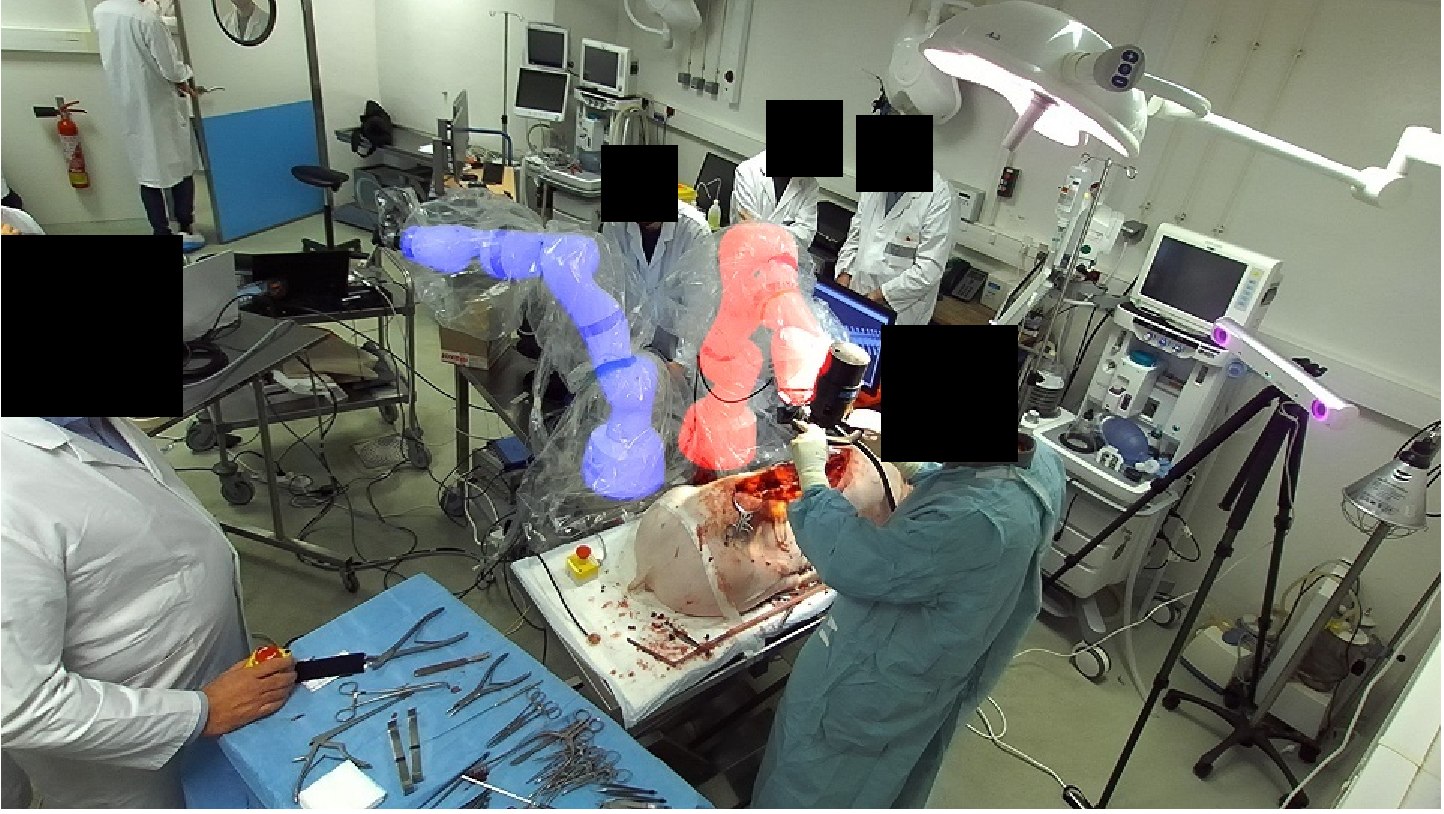
\includegraphics[width=\textwidth]{conclusion/img/draped_ground_truth.pdf}
    \caption{Caption. Refers to \secref{con:sec:marker_free}.}
    \label{con:fig:draped_ground_truth}
\end{figure}
- less dependencies, test of time
- differentiable rendering -> solving draped robots

\section{Homography-based Visual Servo with Remote Center of Motion Constraint}
\label{con:sec:visual_servo}
\paragraph{Contributions} In \chapref{chap:robotic_endoscope}, we introduced a novel image-based visual servoing approach with RCM constraint. We attempted to shift the control paradigm from a tool-centric control policy towards a view-centric control policy to address the flaws of the dominant visual servos, refer \secref{in:sec:rule_based_approaches}, \figref{in:fig:com}. To this end, we derived a homography-based visual servo which does not rely on depth nor on tool distance for inferring actions \figref{c2:fig:schematic}. We did so, introducing a projection operator for mapping target camera frame velocities to available DOF, \eqref{c2:eq:proj}. We then deployed the newly derived control in a novel view-graph-based semi-autonomous scheme on a real system, see \figref{c2:fig:pipe}, \figref{in:fig:experimental_setup}. The proposed method demonstrated good image space convergence properties throughout traversing the view graph from current to target view whilst retained a deviation from the target RCM below $5\,\text{mm}$, see \figref{c2:fig:errors}. The proposed method further indicated robustness against patient re-positioning, i.e. coordinate system change, see \tabref{c2:tab:repositioning}.

\paragraph{Shortcomings and Future Work} The most apparent shortcoming of the proposed method is the assumption of a mostly static surgical scene which clearly does not hold, see \figref{c2:fig:tool_insertion_trajectory}. This temporality assumption, however, is not so crucial within the overarching context of the thesis, as ultimately the executed action is not graph-based but rather incrementally sampled from a learned expert policy $\pi_\text{E}:\, \hat{s}_t \rightarrow \hat{a}^*_t$, refer \secref{in:sec:imitation_learning}. A shortcoming that weighs much heavier is e.g. the lack of force sensing. No trocar-laparoscope external forces nor arm-environment external forces are incorporated into the controller. Arm-environment external forces could e.g. be minimized through nullspace projection and the redundant DOF of the manipulator. The proposed controller furthermore does not explicitly constrain solutions to the RCM, and convergence to undesired minima might occur. Further research should thus introduce constrained optimization instead.

\paragraph{Key Takeaway} Altogether, it was demonstrated that indeed the introduced visual servo could serve as means for executing actions $\hat{a}^*_t$ for the hypothesized pipeline, refer \figref{in:fig:hypothesized_pipeline}, but that future improvements would be necessary for successful clinical translation.

\section{Homography-based Camera Motion Estimation}
\label{con:sec:hom_est}
\paragraph{Contributions} In \chapref{chap:camera_motion_extraction}, we introduce a novel data augmentation \algoref{c3:alg:hom} for runtime generation of synthethic camera motion, see \figref{c3:fig:hom}. We introduce a new dataset of camera motion separated da Vinci\textsuperscript{\textregistered} surgery image sequences through exploitation of the clamping mechanism, which we initially proposed in \figref{in:fig:camera_motion}. Therefore, we utilize all available high frame rate datasets from \tabref{in:sec:search_for_available_data} and summarize their respective sizes in \figref{c3:fig:data}. We conduct an extensive backbone search for models that are regressed onto the synthetic data across multiple compute regimes and devices, \tabref{c3:tab::results}. For evaluating the transferability from videos of RMIS to MIS, we hand-annotate static landmarks in video sequences of laparoscopic interventions \figref{c3:fig:seg}. We find that models which are supervisedly trained on the novel dataset with the novel \textit{homography generation algorithm} outperform classical feature-based homography estimators. We find that they only outperform classical methods when trained on sequence lengths $N>1$, see \figref{c3:fig:resnet34}, justifying our proposed approach. We further find that the learned models outperform the feature-based ones across varying edge deviations $\varrho$. A quantitative statistical significance is shown in \figref{c3:fig:resnet34_c}. Qualitatively we find that static vessels in the background are aligned better through our novel approach, \figref{c3:fig:qualitative}.

\paragraph{Shortcomings and Future Work}
\begin{figure}[tb]
    \centering
    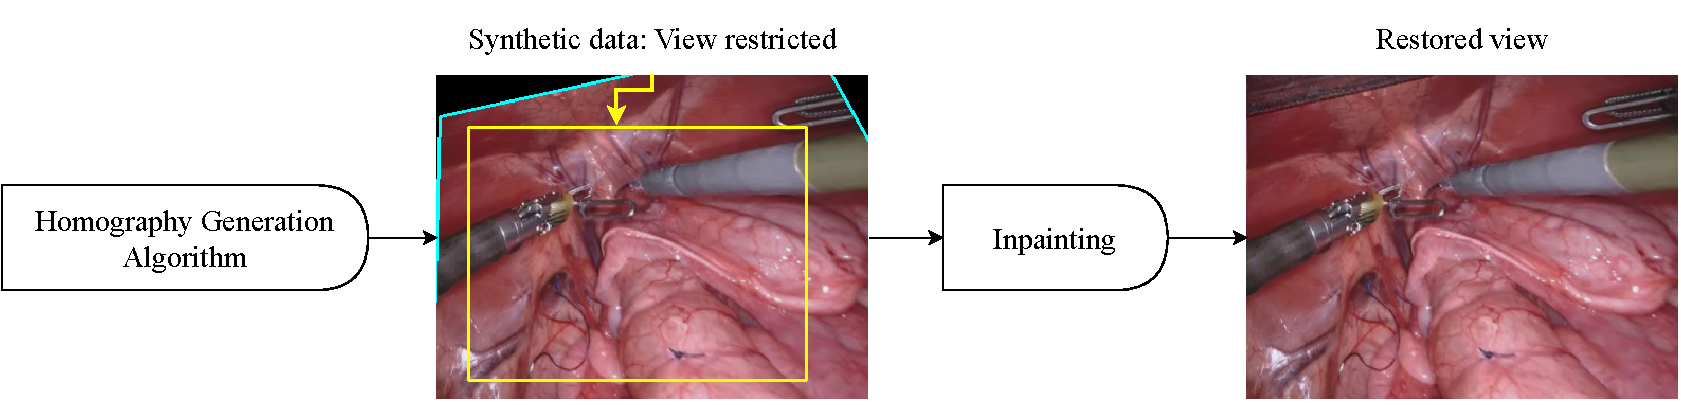
\includegraphics[width=\textwidth]{conclusion/fig/fourier_inpainting.pdf}
    \caption{Proposed inpainting for data retrieval. The \textit{homography generation algorithm} from \secref{c3:sec:hom_gen}, \figref{c3:fig:hom}, introduces black boundaries and thus restricted views. Generative inpainting could help restore the entire view. Fourier inpainting done via \cite{suvorov2021resolution}, \textbf{not} fine-tuned. Refers to \secref{con:sec:hom_est}.}
    \label{con:fig:inpainting}
\end{figure}
Whilst significant improvements are demonstrated over state of the art homography estimates, there still exist shortcomings of this work. The \textit{homography generation algorithm}, although capable of generating indefinite synthetic camera motion, introduces the necessity to crop the view as otherwise black borders would be introduced. This intrinsically limits the magnitude of synthetic camera motion and therefore also the range of learnable camera motion. This fact is somewhat underevaluated through the hand-annotations from \figref{c3:fig:seg} as images were annotated on a frame-to-frame basis with relatively little camera motion in-between. For future work, we suggest to train a generative inpainting model that restores the entire view post camera motion generation, see \figref{con:fig:inpainting}. In this example, an unrefined inpainting model was utilized, showcasing the feasibility of dedicated methods. We suggest the use of a standard generative approach as opposed to diffusion models, such as \cite{rombach2022high}, since the iterative process might not satisfy the runtime requirements of the \textit{homography generation algorithm}. Furthermore, future research might aim at incorporating depth information for camera motion synthesis, e.g. through \cite{budd2024transferring}.

\paragraph{Key Takeaway} \chapref{chap:camera_motion_extraction} introduced several novelties for estimating camera motion in dynamic surgical scenes despite the presence of tool and organ motion, proving the hypothesized pipeline in \figref{in:fig:camera_motion}. As such, the work presented in \cite{huber2022deep} presents the state of the art methodology for generation of state-action pairs $(\hat{s}_t, \hat{a}^*_t)$, refer \secref{in:sec:imitation_learning}, to be used in the imitation learning proposal of \figref{in:fig:hypothesized_pipeline}.

\section{Homography-based Camera Motion Prediction}
\label{con:sec:hom_pred}


\paragraph{Contributions} In \chapref{chap:camera_motion_prediction},  
\paragraph{Shortcomings and Future Work}
\paragraph{Key Takeaway}


- rl on-top (force controlled rcm, rlhf)
- bootstrapping motion:
    - visual qa
- llm interface models: \figref{in:fig:hypothesized_pipeline} (beyond scope)


\section{Closing Remarks}
And therefore Bayern Munich is better than Manchester United.

%the proposed pipeline holds an interesting framework for self-supervised .... indeed proving that \figref{in:fig:auxiliary_tasks}
